%!TEX root = ../main.tex
% What is the project about? 
% What problem are you tackling? 
% What is your research question? 
% Why do these problems need solutions? Why are they important?
% What is the background to the problem? Who is the client? What do they want?
% What existing methods have been tried? How has I.T. been applied so far? 
% What constraints do you have? (Time, PCs, money, users, software, etc) 
% What is the scope of what you have set yourself to do. What is not included?
% What broad approach was taken? (Summarise your broad approach the project) 

\chapter{Introduction}
\label{chap:intro}
% Building context
This chapter will begin by introducing the issue to be addressed throughout
this dissertation, stating the current situation and looking at it from the
perspective of existing solutions. The following section outlines the project
rationale and presents the intended outcomes. The next section states the
objectives and relationship between them, after which it details the method of
critically evaluating the project's success criteria. The penultimate section
describes the risk analysis performed and the proactive actions which will be
taken to mitigate the identified risks. Finally, the last section presents an
overview of the remaining chapters of the dissertation.

\begin{figure}[b]
	\centering
	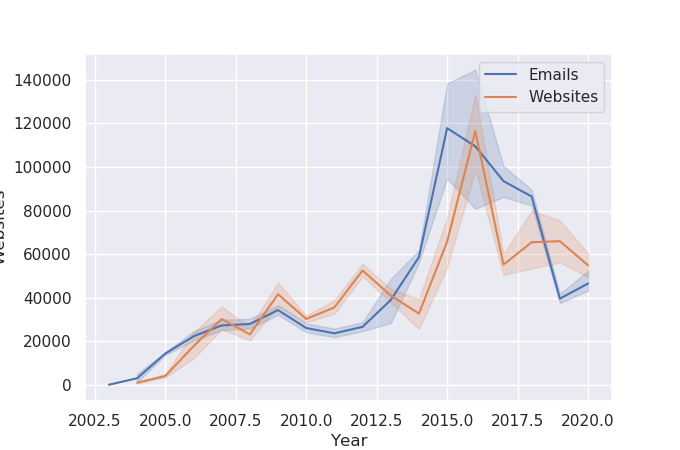
\includegraphics[width=0.49\textwidth]{apwg_attack_hist.png}
	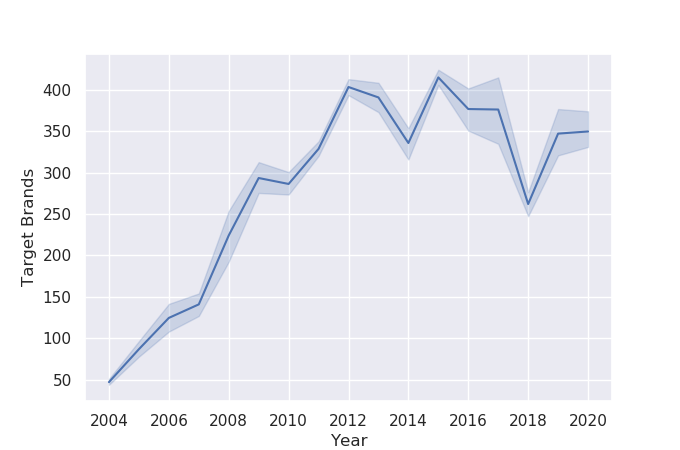
\includegraphics[width=0.49\textwidth]{apwg_brands_hist.png}
	\caption{Phishing attacks over the years (Emails, Websites and Brands
		targeted)}
	\label{fig:PHISHING_HISTORY}
\end{figure}

\section{Problem definition}
% Discuss statistics and identity theft
While the exploitation of trust or personality traits such as agreeableness or
obedience is not a new phenomenon, the internet has brought about a new
framework in which such activities can be conducted. Comparing the
aforementioned to a face-to-face setting, the former provides several advantages
for the attacker such as anonymity and a greater geographical reach. Once with
this contextual shift, the term "phishing" has been popularized. Phishing is
described as a scam by which an internet user is manipulated into disclosing
personal or confidential information that the attacker can use illicitly
\citep{MERRIAM_WEBSTER}.

In its primitive form, a phishing attack requires elementary technical
knowledge. The main skills required are the ones easily transferable from
manipulation or deceit in face-to-face interaction. This amongst other reasons
outlined in the following subsections, has contributed to the growth in
popularity of phishing attacks in the past twenty-five years.

\subsection{Current situation}
The increase in popularity of phishing is seen in the numbers registered by the
Anti-Phishing Working Group \citep{APWG} across the years. Their archives open
with the reports from 2004 adding up to 33.5 thousand unique phishing attacks
with missing data for September. After fifteen years, the APWG registered
479,468 unique phishing attacks in 2019. Besides the growth in numbers, the
aforementioned reports outline a clear advancement in the technical aspects of
the registered phishing campaigns over the years. An example of evolution is the
adoption of Transport Layer Security (TLS) used to serve phishing websites over
HTTPS. Reported usage has grown from close to zero percent in 2016, to
sixty-eight percent by the end of the third quarter of 2019 \citep{APWG_Q42019}.

\subsection{Existing solutions}
% (how do solutions deal with phishing and why is it not working) 
% https://gs.statcounter.com/
In most cases, the only source of protection against accessing phishing websites
the user has is the browser. The browser usage statistics show that Google
Chrome, Apple Safari, and Mozilla Firefox comprise 86.01\% of the market share.
All of these browsers use Google Safe-Browsing as their anti-phishing detection
system. At the surface level, this is a black-list based service which rovides
the aforementioned browsers with a list of malicious URLs through its
Application Programming Interface (API).

% Figure showing browser market share
% Look at issues with Google Safe-Browsing

Although Google Safe Browsing acts as a black-list, underneath this compilation
of malicious URLs lies an entire process of scrutinization. Based on it, the
decision-making mechanism chooses whether the URL of the studied web page should
be added to the black-list. Because of the time needed for this process to
finalize and update the list, this solution can be labeled as suboptimal. The
core issue is that attackers are quick in conducting these phishing attacks and
often go under Google Safe Browsing's radar. This is reflected in the reported
average lifespan of a phishing webpage.

The maintenance of this type of list is resource-expensive. This could be the
reason why three of the major browsers are using the same anti-phishing solution
despite its effectiveness. In conclusion, the user's main defense against
phishing is not versatile or robust enough to keep up with the speed and
sophistication of these attacks.

% ANTONIA NISOTI ET AL SHOWS THAT MOBILE BROWSERS DO NOT DELIVER THE SAME 
% PROTECTION AS DESKTOP BROWSERS
% Build an appendix of phishing attacks calendar based on APWG and point to it
%or further extract and present information


\section{Project rationale and outcomes}
% Why do this project?

% Proposed solution (What should be the level of detail?)
The trends and statistics outline the fact that phishing will remain a prevalent
type of attack for the foreseeable future. However, the protection
mechanisms of the main medium of interaction with phishing webpages are not
satisfactory, as shown by the amount of financial damage reported every year
\citep{APWG_Q42019}. Furthermore, identity theft is difficult to recover from,
and it takes time and effort.

Given the lack of empirical tests in evaluating browser protection, an
investigation of the effectiveness and accuracy of existing anti-phishing
detection systems needs to be carried out. This evaluation and research aimed at
the inner workings of these solutions serve as a starting point for developing
an improvement. As a next step, the relevant literature should be corroborated
and the most appropriate solutions stacked together and implemented. The said
implementation is meant to either outperform existing systems or complement them
to achieve an overall greater level of protection.

To the best of my knowledge, there has been no other approach structured as
described previously, which comprises the motivation of the project. There are
not many iterations of anti-phishing detection systems targeting users with
reduced technical literacy.
% TO BE REVISITED

\section{Aim and objectives}

\subsection{Aim}
The intended functional outcome of the project is a piece of software that
addresses some of the issues of phishing detection systems described in this
chapter. The first step in doing so is to develop the means to evaluate the
efficiency of Google Safe Browsing, this being the most used anti-phishing
detection system. The second step will be composed of research, design, and
development of an improved solution.

\begin{landscape}
	\begin{singlespace}
		\subsection{Objectives}
		\begin{center}
			\label{tab:OBJECTIVES}
			\begin{tabular}{ | m{0.5em} | m{18.5em} | m{23em}| m{16em} | }
				\hline
				\textbf{\#} & \textbf{Objective} & \textbf{Objective actions} &
				\textbf{Success criteria}                                       \\
				\hline
				\textbf{1}  &
				To research and develop a mechanism for evaluating the
				accuracy of phishing detection systems embedded in popular
				browsers.
				            &
				1. Research how the browser phishing detection systems and
				warnings working
				\newline\newline
				2. Find the appropriate tools and/or libraries to automate the
				process of evaluation
				\newline\newline
				2. Enter a design, development and evaluation loop until the
				automation script proves to be reliable
				            &
				The final product evaluates the phishing detection system of
				browsers with a minimal error margin.                           \\


				\hline
				\textbf{2}  &
				To  research and corroborate different anti-phishing methods
				described in the literature into a multi-layered phishing
				detection design.
				            &
				1. Research different approaches towards phishing detection
				systems
				\newline\newline
				2. Build an educated selection of features and design the
				high-level overview of the system to be implemented
				            &
				The final product evaluates the phishing detection system of
				browsers with a minimal error margin.                           \\


				\hline
				\textbf{3}  &
				To implement and calibrate a phishing detection system that
				improves the status quo and can be operated with minimal
				technical literacy
				            &
				1. Enter a software design, development, and evaluation loop to
				implement every non-machine learning feature selected in the
				research phase
				\newline\newline
				2. Train the machine learning algorithms and review their
				efficiency in carrying out the designated tasks
				\newline\newline
				3. Stack the solutions and evaluate system performance,
				efficiency, and ease of use
				            &
				The solution developed either surpasses or complements popular
				browser anti-phishing mechanisms in achieving a better success
				rate.                                                           \\

				\hline
			\end{tabular}
			\captionsetup{type=table}\caption{Objectives list}
		\end{center}
	\end{singlespace}
\end{landscape}
\section{Risk Analysis}

Considering the nature of this dissertation and the extensive amount it
plans to achieve, a risk analysis is a useful resource. This will assure a
proactive stance regarding the obstacles that are to be encountered. Besides the
resilience it offers, it helps in acknowledging areas where problems may arise
and prioritize work items based on this.

Table \ref{tab:RISK_ANALYSIS} presents the main identified risks related to
this project. Each of these has a likelihood and impact dimension attributed to
help outline the hierarchy of prioritization.

\begin{singlespace}
	\begin{center}
		\label{tab:RISK_ANALYSIS}
		\begin{tabular}{ | m{0.5em} | m{7em} | m{5em} | m{3.2em}| m{17.5em} | }
			\hline
			\textbf{\#} & \textbf{Description} & \textbf{Likelihood} & \textbf{Impact} & \textbf{Intended mitigation} \\
			\hline
			\textbf{1}  &
			Time management issues
			            &
			Medium
			            &
			High
			            &
			Develop a plan and Gantt chart before starting the dissertation.
			Calculate the amount of time necessary to accomplish project's
			objectives and add an arbitrary error margin to it.                                                       \\
			\hline
			\textbf{2}  &
			Sub-optimal solution results
			            &
			Medium
			            &
			High
			            &
			Allocate more time for the phishing detection system development
			than the estimated necessary. This is to calibrate and improve the
			solution's efficiency and performance                                                                     \\
			\hline
			\textbf{3}  &
			Fatigue, anxiety or health issues
			            &
			Medium
			            &
			High
			            &
			The first two are highly influenced by time management which has
			been covered. Health issues will be prevented by following a healthy
			lifestyle and restrict interactions with contagious people.                                               \\
			\hline
			\textbf{4}  &
			Inaccurate assumptions
			            &
			High
			            &
			Low
			            &
			Extensive research is being done at every step of the dissertation.
			This is done to reduce the number of assumptions and base the work
			only on educated ones                                                                                     \\
			\hline
			\textbf{5}  &
			Data loss
			            &
			Low
			            &
			High
			            &
			Throughout the dissertation development, the back-up rule of 3-2-1
			will be followed. This issue dictates that three copies of the data
			should be stored on at least two mediums of storage, one being
			off-site.                                                                                                 \\
			\hline
			\textbf{6}  &
			Chosen tools are not appropriate for the task
			            &
			Low
			            &
			High
			            &
			Do brief or comprehensive background checks for all the tools and
			libraries used in the project depending on their importance to the
			success of the project. At the same time not using more tools or
			libraries than strictly necessary                                                                         \\
			\hline
		\end{tabular}
		\captionsetup{type=table}\caption{Risk analysis}
	\end{center}
\end{singlespace}

\section{Overview of the dissertation}
Chapter two explores the relevant literature and introduces previous work done
on the subject. Chapter three will describe the methodology used in designing
and implementing the artifact, as well as the process of developing the browser
evaluation scripts and the artifact evaluation process. Chapter four offers an
in-depth view of the requirements and requirements analysis. Furthermore, it
will illustrate the expansion fo the objectives into requirements. The fifth
chapter will follow the process of design and implementation of the artifact and
adjacent software. The last chapter will outline the outcomes of the
dissertation and close the is with a summarization of the work, presented as a
conclusion.





% =========================================================================================================
% Skipped compiling instructions
\iffalse
	\section{BU Template}
	The text within the square brackets must be deleted along with the square brackets when finalising your chapters.

	This is only a guidance template. Depending on the nature of your project, the structure of your dissertation is open to discussion. Please check with your supervisor if you are not sure.

	Arial, Normal, 11pt with 1.2 or 1.5 line spacing should be used in the main body. The text in this part has 1.5 line spacing.

	Figures must be correctly numbered with captions and paragraph text should not be wrapped around figures - same rules apply to tables. An example of figures can be found below.
	\begin{figure}[t]
		\centering
		
\includegraphics[width=0.45\textwidth]{unilogo.jpg}
		\caption{Bournemouth University}
		\label{fig:BULogo1}
	\end{figure}
	The Introduction chapter should cover the following using Heading 2 style:
	\begin{itemize}
		\item Background and context (e.g., who is your client, what is the problem, why this needs to be solved (impact), what does your client want you to do)
		\item Proposed solution (e.g., what is proposed to solve the problem) – note you should not include too many technical details, you should tell what the client is expecting from you
		\item Aims and objectives – note the SMART for objectives
		\item Success criteria – for each objective
		\item Risk analysis – a summary table must be provided with all risks and solutions.
		\item Overview of dissertation/Remaining chapters]
	\end{itemize}
\fi

